\section{El DUNE verso: módulos}

\begin{frame}[fragile]
	\frametitle{\secname}
	\framesubtitle{\url{https://dune-project.org/groups/core}}

	\begin{figure}[ht!]
		\centering
		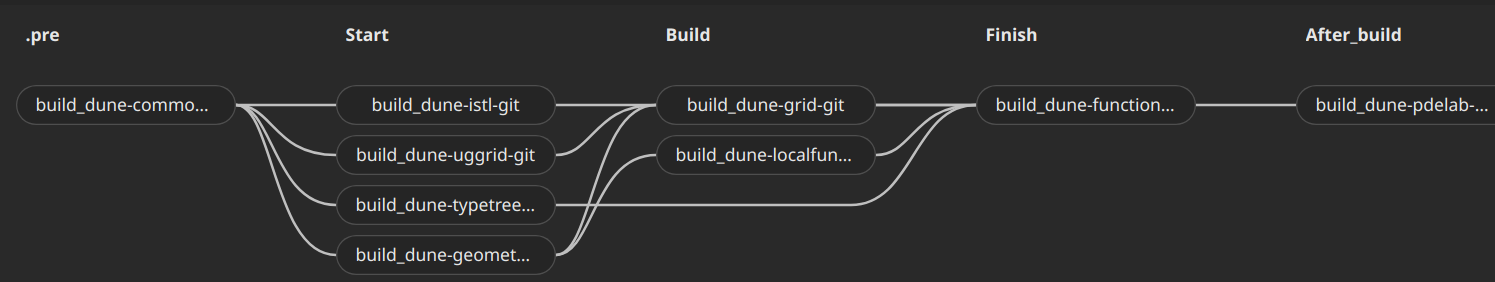
\includegraphics[width=14.6cm]{dependences}
		\caption*{
			\textbf{Origen:}~\url{https://gitlab.com/dune-archiso/repository/dune-archiso-repository-pdelab-git/-/pipelines}.
		}
	\end{figure}

	\begin{description}
		\item[\href{https://dune-project.org/modules/dune-common}{dune-common}]

			Clases fundamentales e infraestructura para la construcción del
			sistema.

		\item[\href{https://dune-project.org/modules/dune-geometry}{dune-geometry}]

			Elementos de referencia, métodos de cuadraturas y
			transformaciones geométricas.

		\item[\href{https://dune-project.org/modules/dune-grid}{dune-grid}]

			Interfaces con las mallas
			(\href{https://dune-project.org/modules/dune-alugrid}{ALUGrid},
			\href{https://dune-project.org/modules/dune-uggrid}{UGGrid},
			\href{https://dune-project.org/modules/dune-grid}{AlbertaGrid, YaspGrid}).
			% , construcción y visualización

		\item[\href{https://dune-project.org/modules/dune-istl}{dune-istl}]

			Biblioteca de solucionadores iterativas de plantillas, clases
			genéricas de matrices/vectores dispersos.
			%, solucionadores

		\item[\href{https://dune-project.org/modules/dune-localfunctions}{dune-localfunctions}]

			Interface genérica para funciones de elementos finitos.
	\end{description}

	\note{
		\begin{description}
			\item[dune-common]

				Contiene las clases base usadas por todos los módulos de
				DUNE-módulos.

				Provee algunas clases de infraestructura para depuración y
				manejo de excepciones así como una librería para manejar una
				matriz densa y vectores.

			\item[dune-grid]

				Define mallas jerarquizadas, paralelas, de dimensiones
				arbitrarias, permite salida a formatos que puedens ser leídos
				por ParaView.
		\end{description}
	}
\end{frame}

\subsection{Dependencias de algunos módulos}

\begin{frame}
	\frametitle{\secname}
	\framesubtitle{\subsecname}
	\small
	\begin{columns}
		\begin{column}{0.5\textwidth}
			\dirtree{%
				.1 dune-fem.
				.2 dune-alugrid.
				.2 dune-istl.
				.2 dune-localfunctions.
				.2 \href{https://github.com/FEniCS/ufl}{python-fenics-ufl}.
				.2 \href{https://matplotlib.org}{python-matplotlib}.
				.2 \href{https://scipy.org}{python-scipy}.
				.2 dune-polygongrid (opcional).
				.2 dune-spgrid (opcional).
				.2 \href{https://eigen.tuxfamily.org}{eigen} (opcional).
				.2 \href{http://icl.cs.utk.edu/papi}{papi} (opcional).
			}


			\dirtree{%
				.1 opm-models.
				.2 dune-alugrid.
				.2 dune-localfunctions.
				.2 opm-grid.
				.3 opm-common.
				.3 \href{http://faculty.cse.tamu.edu/davis/suitesparse.html}{suitesparse}.
				.3 \href{https://github.com/sandialabs/zoltan}{zoltan}.
				.2 dune-fem (opcional).
			}
		\end{column}

		\begin{column}{0.5\textwidth}
			\dirtree{%
				.1 dumux.
				.2 dune-grid.
				.2 dune-istl.
				.2 dune-localfunctions.
				.2 dune-alugrid (opcional).
				.2 dune-foamgrid (opcional).
				.2 dune-functions (opcional).
				.2 dune-mmesh (opcional).
				.2 dune-spgrid (opcional).
				.2 dune-subgrid (opcional).
				.2 opm-grid (opcional).
			}

			\

			\dirtree{%
				.1 dune-pdelab.
				.2 \href{http://reuter.mit.edu/software/arpackpatch}{arpack++}.
				.2 dune-alugrid.
				.2 dune-functions.
				.2 \href{http://faculty.cse.tamu.edu/davis/suitesparse.html}{suitesparse}.
				.2 \href{https://github.com/xiaoyeli/superlu}{superlu}.
				.2 dune-multidomaingrid (opcional).
			}
		\end{column}
	\end{columns}

	\note{
		Aquí se puede ver la relación de dependencias entre los módulos
		de Dune.
	}

\end{frame}
% \href{https://www.boost.org}{boost}.
% \href{https://fmt.dev}{fmt}.